\documentclass[aspectratio=169]{beamer}

\usepackage[utf8]{inputenc}
\usetheme{Singapore}
\usepackage{xcolor}
\setbeamertemplate{footline}[frame number]

\usepackage{amsmath,amssymb,amsthm}
\usepackage{tikz}
\usetikzlibrary{arrows.meta,decorations.pathreplacing}
\usepackage{times}

\input{../sty/macros}

\setbeamercovered{dynamic}

\newtheorem{theo}{Theorem}

% Same shorthands as deck 03, so that the cross-references read identically.
\newcommand{\WS}{\mathrm{WS}}
\newcommand{\EV}{\mathrm{EV}}
\newcommand{\EVPI}{\mathrm{EVPI}}
\newcommand{\VSS}{\mathrm{VSS}}
\providecommand{\bxi}{\boldsymbol{\xi}}

\author[Fabian Bastin]{Fabian Bastin \\ \texorpdfstring{\url{fabian.bastin@umontreal.ca}}{fabian.bastin@umontreal.ca} \\ Université de Montréal -- CIRRELT -- IVADO}
\date{}
\title[Probability]{Probability and statistics\\Background material}

\begin{document}

\frame{\titlepage}

\begin{frame}
\frametitle{What this deck is for}

The course assumes a working knowledge of probability. This deck collects the notions it actually uses, and nothing more.

\begin{center}
{\footnotesize
\begin{tabular}{|l|l|}
\hline
Notion & Where the course needs it \\
\hline
\hline
Probability space, measurability & $\calQ(x)$ is well defined (deck~03) \\
Support $\Xi$ & $K_2$, $K_2^P$, scenario trees (decks~03, 06) \\
Quantile $F^{-1}$ & inversion sampling (deck~02), chance constraints (deck~05) \\
Expectation, {\red second-order moments} & nearly every theorem of decks~03--04 \\
Jensen's inequality & $\EV \leq \WS$ (deck~03) \\
``almost surely'' & $K_2$ versus $K_2^P$ (deck~03) \\
Conditional expectation & multistage, non-anticipativity (decks~06--08) \\
Modes of convergence, LLN & sample average approximation (deck~09) \\
Central limit theorem, CIs & stopping rules (decks~07, 10, 12) \\
\hline
\end{tabular}}
\end{center}

Throughout, {\red $\bsxi$} denotes a random vector and {\red $\xi$} one of its realizations --- the convention used in the slides.

\end{frame}

%%%%%%%%%%%%%%%%%%%%%%%%%%%%%%%%%%%%%%%%%%%%%%%%%%%%%%%%%%%%%%%%%%%%%%%%%%%%%%

\begin{frame}
\frametitle{Probability space}

A {\red probability space} is a triplet $(\Omega, \calF, P)$:
\begin{enumerate}
\item
$\Omega$ is the {\red sample space}, an arbitrary non-empty set;
\item
$\calF \subseteq 2^{\Omega}$ is a {\red $\sigma$-algebra} (or $\sigma$-field): a collection of subsets of $\Omega$, called {\red events}, such that
\begin{itemize}
	\item $\Omega \in \calF$,
	\item $A \in \calF \Rightarrow \Omega \backslash A \in \calF$,
	\item $A_i \in \calF$, $i = 1, 2, \ldots \Rightarrow \bigcup_i A_i \in \calF$;
\end{itemize}
\item
$P: \calF \rightarrow [0,1]$ is a {\red probability measure}: $P[\Omega] = 1$, and
$P\left[\bigcup_i A_i\right] = \sum_i P[A_i]$ for any countable collection of pairwise disjoint $A_i \in \calF$.
\end{enumerate}

\mbox{}

An event $A$ {\it occurs} if the outcome $\omega$ of the experiment belongs to $A$.

\end{frame}

\begin{frame}
\frametitle{Why a $\sigma$-algebra?}

Why not simply take $\calF = 2^{\Omega}$, and give every subset a probability?

\mbox{}

Because on an uncountable $\Omega$ --- say $[0,1]$ --- no probability measure can assign a consistent value to {\it every} subset. One has to restrict attention to a family that is rich enough to be useful and small enough to be consistent. That family is a $\sigma$-algebra, and its members are exactly the sets we are allowed to call events.

\mbox{}

Two consequences that matter for the course:
\begin{itemize}
\item
a function of $\omega$ is only usable if it is {\red measurable} --- otherwise ``$P[\bsxi \leq x]$'' is meaningless;
\item
in deck~03, the measurability of $Q(x,\bsxi)$ is what makes $\calQ(x) = \EE_{\bsxi}[Q(x,\bsxi)]$ well defined at all. It is assumed, not proved, there.
\end{itemize}

\mbox{}

For a finite or countable $\Omega$, $\calF = 2^{\Omega}$ causes no trouble, and this discussion can be ignored: that is the setting of most scenario-based models.

\end{frame}

\begin{frame}
\frametitle{Random variables and random vectors}

A {\red random variable} $\bsxi$ on $(\Omega, \calF, P)$ is a function $\xi(\omega)$, $\omega \in \Omega$, such that
\[
\lbrace \omega \,|\, \xi(\omega) \leq x \rbrace \in \calF \quad \text{for every } x \in \RR,
\]
so that a probability can be attached to $\lbrace \bsxi \leq x \rbrace$. A {\red random vector} $\bsxi: \Omega \rightarrow \RR^r$ is defined componentwise.

\mbox{}

Its {\red cumulative distribution function} (cdf) is
\[
F_{\bsxi}(x) = P[\bsxi \leq x].
\]

\mbox{}

The {\red support} $\Xi \subseteq \RR^r$ of $\bsxi$ is the {\red smallest closed set} with $P[\bsxi \in \Xi] = 1$.

\mbox{}

{\footnotesize The closedness in that definition is not a detail: it is exactly what makes the argument of deck~03 work, where a set of favourable $\xi$ that is closed and of probability one must contain the whole support.}

\end{frame}

\begin{frame}
\frametitle{Discrete and continuous random variables}

{\red Discrete}: $\bsxi$ takes finitely or countably many values $\xi_k$, with {\red probability masses} $p_k = P[\bsxi = \xi_k]$, $\sum_k p_k = 1$. This is the {\it scenario} setting of the course.

\mbox{}

{\red Continuous}: $\bsxi$ admits a {\red density} $f$, and then $P[\bsxi = x] = 0$ for every $x$, while
\[
P[a \leq \bsxi \leq b] = \int_a^b f(x)\,dx = \int_a^b dF(x) = F(b)-F(a).
\]

\mbox{}

Writing $dF$ rather than $f(x)dx$ covers both cases at once, and is the notation the slides use.

\mbox{}

{\footnotesize A distribution need be neither of the two: a discrete part and a density can coexist. Nothing in the course requires that generality, but the $dF$ notation handles it.}

\end{frame}

\begin{frame}
\frametitle{Distribution function and quantiles}
\small

From its definition, $F_{\bsxi}$ takes values in $[0,1]$, is non-decreasing, and tends to $1$ at $+\infty$ and to $0$ at $-\infty$.

The {\red quantile function} is the {\red generalized inverse}
\[
F_{\bsxi}^{-1}(p) = \inf \lbrace x \in \RR \,|\, F_{\bsxi}(x) \geq p \rbrace, \quad p \in (0,1),
\]
which is defined whether or not $F_{\bsxi}$ is invertible --- in particular for discrete variables, where $F$ has jumps.

\mbox{}

{\blue Two uses in the course.} If $\bsxi$ is continuous, $F_{\bsxi}$ is continuous and invertible on $\Xi$, so for $u \in [0,1]$,
\[
P[F_{\bsxi}(\bsxi) \leq u] = P\left[\bsxi \leq F_{\bsxi}^{-1}(u)\right] = F_{\bsxi}\left(F_{\bsxi}^{-1}(u)\right) = u,
\]
i.e. $F_{\bsxi}(\bsxi) \sim U[0,1]$. Read backwards, this is {\red inversion sampling} (deck~02); and a chance constraint $P[\cdot] \geq \alpha$ is a statement about a quantile (deck~05).

\end{frame}

\begin{frame}
\frametitle{Cdf, quantile and support, graphically}
\small

\begin{center}
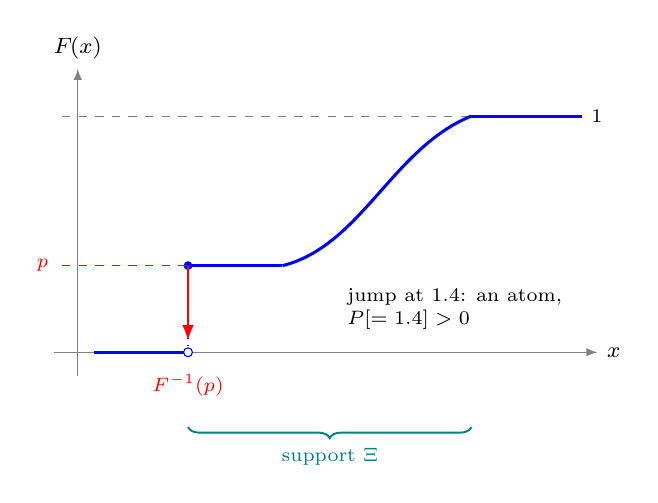
\begin{tikzpicture}[x=1cm,y=1cm,>=latex,font=\footnotesize]
  % axes
  \draw[->,gray] (-0.3,0) -- (6.6,0) node[right,black]{$x$};
  \draw[->,gray] (0,-0.3) -- (0,3.6) node[above,black]{$F_{\bsxi}(x)$};
  \draw[dashed,gray] (-0.2,3) -- (6.4,3) node[right,black,font=\scriptsize]{$1$};
  % a mixed cdf: flat, jump, slope, flat
  \draw[blue,line width=1.1pt] (0.2,0) -- (1.4,0);
  \draw[blue,line width=1.1pt] (1.4,1.1) -- (2.6,1.1);
  \draw[blue,line width=1.1pt] (2.6,1.1) .. controls (3.6,1.35) and (4.0,2.6) .. (5.0,3);
  \draw[blue,line width=1.1pt] (5.0,3) -- (6.4,3);
  \draw[blue,dotted] (1.4,0) -- (1.4,1.1);
  \fill[blue] (1.4,1.1) circle (1.6pt);  \draw[blue,fill=white] (1.4,0) circle (1.6pt);
  % quantile read-off
  \draw[red,dashed] (-0.2,1.1) -- (1.4,1.1);
  \node[red,left,font=\scriptsize] at (-0.25,1.1) {$p$};
  \draw[->,red,line width=0.9pt] (1.4,1.1) -- (1.4,0.15);
  \node[red,below,font=\scriptsize] at (1.4,-0.15) {$F^{-1}_{\bsxi}(p)$};
  % support
  \draw[decorate,decoration={brace,mirror,amplitude=4pt},teal,line width=0.7pt] (1.4,-0.95) -- (5.0,-0.95);
  \node[teal,below,font=\scriptsize] at (3.2,-1.1) {support $\Xi$};
  \node[align=left,font=\scriptsize,anchor=west] at (3.3,0.55)
     {jump at $1.4$: an atom,\\$P[\bsxi = 1.4] > 0$};
\end{tikzpicture}
\end{center}

{\footnotesize A flat stretch of $F$ is a region the variable never visits; a jump is an atom. The quantile is read horizontally then downwards, the $\inf$ picking the left end of a flat stretch. The support is the closure of what is left.}

\end{frame}

%%%%%%%%%%%%%%%%%%%%%%%%%%%%%%%%%%%%%%%%%%%%%%%%%%%%%%%%%%%%%%%%%%%%%%%%%%%%%%

\begin{frame}
\frametitle{Expectation}
\small

\[
\EE[\bsxi] = \sum_k p_k \xi_k \quad \text{(discrete)}, \qquad
\EE[\bsxi] = \int_{-\infty}^{+\infty} x f(x)\,dx = \int_{-\infty}^{+\infty} x\,dF(x) \quad \text{(continuous)}.
\]

\mbox{}

More useful in practice: for a measurable $g$,
\[
\EE[g(\bsxi)] = \int_{\Xi} g(x)\,dF(x),
\]
{\red without} having to know the distribution of $g(\bsxi)$. This is what allows the course to write $\calQ(x) = \EE_{\bsxi}[Q(x,\bsxi)]$ directly.

\mbox{}

Expectation is {\red linear}: $\EE[a\bsxi + b\bseta] = a\EE[\bsxi] + b\EE[\bseta]$, whether or not $\bsxi$ and $\bseta$ are independent.
It is {\red monotone}: $\bsxi \leq \bseta$ a.s. $\Rightarrow \EE[\bsxi] \leq \EE[\bseta]$.

\mbox{}

{\footnotesize Both are used constantly and silently in the decks: linearity to split $\EE[c^Tx + q^Ty]$, monotonicity to take expectations of an inequality, as in the proofs of $\EVPI \geq 0$ and $\VSS \geq 0$.}

\end{frame}

\begin{frame}
\frametitle{Variance, covariance, and ``finite second-order moments''}
\small

\[
\var[\bsxi] = \EE\left[(\bsxi - \EE[\bsxi])^2\right] = \EE[\bsxi^2] - \EE[\bsxi]^2,
\qquad
\cov[\bsxi, \bseta] = \EE\left[(\bsxi - \EE\bsxi)(\bseta - \EE\bseta)\right].
\]
For a random vector, the covariance matrix $\Sigma = \EE[(\bsxi-\EE\bsxi)(\bsxi-\EE\bsxi)^T]$ is symmetric positive semi-definite.

\mbox{}

The hypothesis {\red ``$\bsxi$ has finite second-order moments''}, which appears eight times in deck~03 alone, means
\[
\EE\left[\|\bsxi\|^2\right] < \infty,
\]
equivalently: every component has a finite variance.

\mbox{}

{\blue Why the course needs exactly this.} By {\red Cauchy--Schwarz},
\[
\EE\left[\,|\bsu^T\bsv|\,\right] \leq \EE\left[\|\bsu\|\|\bsv\|\right] \leq \left(\EE\|\bsu\|^2\right)^{1/2}\left(\EE\|\bsv\|^2\right)^{1/2}.
\]
In a two-stage model the recourse cost is of the form $q(\bsxi)^Tz(\bsxi)$ with $q$ and $z = h - Tx$ affine in $\bsxi$. Finite second-order moments therefore make $\EE$ of that product finite --- which is precisely what makes $\calQ(x)$ finite, and what the simple-recourse proof of deck~03 invokes.

\end{frame}

\begin{frame}
\frametitle{Independence}

$\bsxi$ and $\bseta$ are {\red independent} if
\[
P[\bsxi \in A,\ \bseta \in B] = P[\bsxi \in A]\, P[\bseta \in B]
\]
for all measurable $A$, $B$; equivalently, their joint cdf factorizes.

\mbox{}

Then $\EE[\bsxi \bseta] = \EE[\bsxi]\EE[\bseta]$ and $\var[\bsxi + \bseta] = \var[\bsxi] + \var[\bseta]$.

\mbox{}

{\red The converse fails}: $\cov[\bsxi,\bseta] = 0$ does not imply independence. Uncorrelated is weaker than independent, except in the Gaussian case where the two coincide.

\mbox{}

{\footnotesize Independence is what justifies $\var[\overline{X}_n] = \sigma^2/n$ for a Monte Carlo average, hence the $1/\sqrt{n}$ rate below. It is also what {\red fails} for the correlated estimators of deck~10, where common random numbers are used deliberately to create a positive correlation and cancel variance in a difference.}

\end{frame}

\begin{frame}
\frametitle{Jensen's inequality}

\begin{theo}
If $\varphi$ is convex and $\bsxi$ is integrable, then
$\varphi\left(\EE[\bsxi]\right) \leq \EE\left[\varphi(\bsxi)\right]$.
For $\varphi$ concave the inequality is reversed.
\end{theo}

\begin{center}
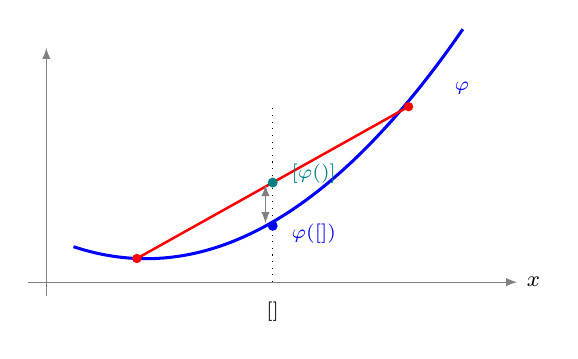
\begin{tikzpicture}[x=1.15cm,y=0.85cm,>=latex,font=\footnotesize]
  \draw[->,gray] (-0.2,0) -- (5.2,0) node[right,black]{$x$};
  \draw[->,gray] (0,-0.2) -- (0,3.5);
  \draw[blue,line width=1.1pt] plot[domain=0.3:4.6,samples=40,smooth] (\x,{0.28*(\x-1.1)*(\x-1.1)+0.35});
  \node[blue,right,font=\scriptsize] at (4.4,2.9) {$\varphi$};
  % two points and the chord
  \draw[red,line width=0.9pt] (1,0.353) -- (4,2.622);
  \fill[red] (1,0.353) circle (1.7pt); \fill[red] (4,2.622) circle (1.7pt);
  % E[xi] = 2.5 ; chord value vs phi value
  \draw[dotted] (2.5,0) -- (2.5,2.6);
  \fill[teal] (2.5,1.4875) circle (1.8pt);
  \fill[blue] (2.5,0.8408) circle (1.8pt);
  \node[below,font=\scriptsize] at (2.5,-0.15) {$\EE[\bsxi]$};
  \node[teal,right,font=\scriptsize] at (2.6,1.62) {$\EE[\varphi(\bsxi)]$};
  \node[blue,right,font=\scriptsize] at (2.6,0.72) {$\varphi(\EE[\bsxi])$};
  \draw[<->,gray] (2.42,0.88) -- (2.42,1.45);
\end{tikzpicture}
\end{center}

\vspace{-1mm}

{\footnotesize With $\bsxi$ taking two values, $\EE[\varphi(\bsxi)]$ sits on the chord and $\varphi(\EE[\bsxi])$ on the curve, below it. Deck~03 uses exactly this to obtain $\EV \leq \WS$: the value function of a linear program is convex in its right-hand side, so replacing $\bsxi$ by its mean can only look {\it too good}.}

\end{frame}

\begin{frame}
\frametitle{``Almost surely'', and why it is not a formality}

An event holds {\red almost surely} (a.s.), or for {\red almost every} $\xi$ (a.e.), if it holds on a set of probability one --- it may fail, but only on a set of probability zero.

\mbox{}

This is not the same as {\it always}, and deck~03 turns the difference into a worked example:
\[
K_2 = \lbrace x \,|\, Q(x,\bsxi) < \infty \text{ {\red a.s.}} \rbrace
\qquad \text{versus} \qquad
K_2^P = \bigcap_{\xi \in \Xi} K_2(\xi) \quad \text{({\red every} $\xi$)}.
\]
A first-stage decision may be infeasible for some realizations, provided they together have probability zero: then $x \in K_2$ but $x \notin K_2^P$.

\mbox{}

With a {\red fixed} recourse the two coincide, because $\lbrace \xi \,|\, x \in K_2(\xi) \rbrace$ is then closed, and a closed set of probability one contains the support. Drop the fixed recourse and they separate --- see the triangular-distribution exercise of deck~03.

\end{frame}

\begin{frame}
\frametitle{Conditional expectation}

For a discrete $\bseta$ with $P[\bseta = e] > 0$,
\[
\EE[\bsxi \,|\, \bseta = e] = \sum_k \xi_k \, P[\bsxi = \xi_k \,|\, \bseta = e],
\qquad
P[A\,|\,B] = \frac{P[A \cap B]}{P[B]}.
\]
In general $\EE[\bsxi \,|\, \calG]$ is defined for a sub-$\sigma$-algebra $\calG \subseteq \calF$: it is the best prediction of $\bsxi$ given the information in $\calG$.

\mbox{}

Two properties carry the multistage chapters:
\begin{itemize}
\item
{\red tower property}: $\EE\left[\EE[\bsxi \,|\, \calG]\right] = \EE[\bsxi]$ --- this is what lets a multistage problem be written recursively, stage by stage;
\item
$\EE[\bsxi \,|\, \calG] = \bsxi$ when $\bsxi$ is $\calG$-measurable, i.e. when $\calG$ already determines $\bsxi$.
\end{itemize}

\mbox{}

{\footnotesize In decks~06--08, $\calG$ is the information available at a given stage. A decision that is $\calG$-measurable is one that uses only what has been observed so far: that is precisely the {\red non-anticipativity} constraint.}

\end{frame}

%%%%%%%%%%%%%%%%%%%%%%%%%%%%%%%%%%%%%%%%%%%%%%%%%%%%%%%%%%%%%%%%%%%%%%%%%%%%%%

\begin{frame}
\frametitle{Modes of convergence}

For random variables $X_n$ and $X$:
\begin{itemize}
\item
{\red almost sure}: $P\left[\lim_n X_n = X\right] = 1$; written $X_n \rightarrow X$ a.s.
\item
{\red in probability}: $P\left[|X_n - X| > \epsilon\right] \rightarrow 0$ for every $\epsilon > 0$.
\item
{\red in $L^2$} (mean square): $\EE\left[(X_n-X)^2\right] \rightarrow 0$.
\item
{\red in distribution}: $F_{X_n}(x) \rightarrow F_X(x)$ at every continuity point of $F_X$; written $X_n \overset{\calD}{\rightarrow} X$ or $X_n \Rightarrow X$.
\end{itemize}

\begin{center}
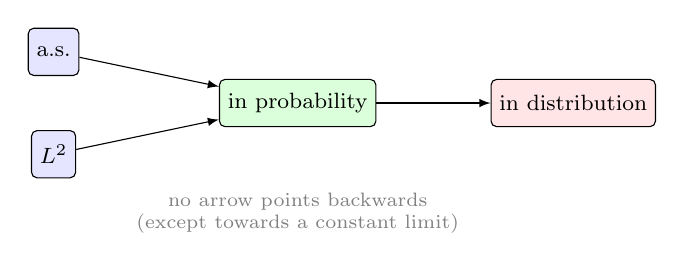
\begin{tikzpicture}[x=1cm,y=1cm,>=latex,font=\footnotesize,
   bx/.style={draw,rounded corners=2pt,inner sep=3pt,minimum height=6mm}]
  \node[bx,fill=blue!10]  (as) at (0,0.8)   {a.s.};
  \node[bx,fill=blue!10]  (l2) at (0,-0.5)  {$L^2$};
  \node[bx,fill=green!14] (pr) at (3.1,0.15) {in probability};
  \node[bx,fill=red!10]   (di) at (6.6,0.15) {in distribution};
  \draw[->] (as) -- (pr);  \draw[->] (l2) -- (pr);  \draw[->] (pr) -- (di);
  \node[font=\scriptsize,gray,align=center] at (3.1,-1.25) {no arrow points backwards\\(except towards a constant limit)};
\end{tikzpicture}
\end{center}

\vspace{-1mm}

{\footnotesize Convergence in distribution to a {\it constant} does imply convergence in probability --- the one reverse implication the course relies on.}

\end{frame}

\begin{frame}
\frametitle{The law of large numbers}
\small

\begin{theo}[Strong law]
If $X_1, X_2, \ldots$ are i.i.d.\ with $\EE[|X_1|] < \infty$, then
\[
\overline{X}_n = \frac{1}{n}\sum_{i=1}^n X_i \longrightarrow \EE[X_1] \quad \text{almost surely.}
\]
\end{theo}

With $X_i = g(x,\xi^i)$ and $\xi^1, \xi^2, \ldots$ an i.i.d.\ sample, this is the whole justification of {\red Monte Carlo}: $\hat{g}_n(x) \rightarrow \EE[g(x,\bsxi)]$ a.s.

{\red But this is pointwise in $x$}, and optimization needs more: the sample average must converge {\it uniformly} over the decision set, otherwise the minimizers need not converge. That stronger statement is the {\red uniform law of large numbers},
\[
\sup_{z \in S} \left| \hat{g}_n(z) - g(z) \right| \longrightarrow 0 \quad \text{a.s.},
\]
and it is the hypothesis on which the whole convergence theory of deck~09 rests.

\end{frame}

\begin{frame}
\frametitle{The central limit theorem}

\begin{theo}
If $X_1, X_2, \ldots$ are i.i.d.\ with mean $\mu$ and {\red finite} variance $\sigma^2$, then
\[
\sqrt{n}\left(\overline{X}_n - \mu\right) \overset{\calD}{\longrightarrow} N(0, \sigma^2),
\quad \text{i.e.} \quad
\overline{X}_n \approx N\!\left(\mu, \frac{\sigma^2}{n}\right) \text{ for large } n.
\]
\end{theo}

The law of large numbers says the estimator converges; the central limit theorem says {\red how fast}, and with which spread.

\mbox{}

Two consequences used throughout the course:
\begin{itemize}
\item
the standard error is $\sigma/\sqrt{n}$: to {\red halve} it, the sample size must be {\red quadrupled}. The $\sqrt{n}$ is not an artefact of the analysis, it is the rate;
\item
the rate does not depend on the dimension of $\bsxi$ --- which is why sampling survives where scenario enumeration explodes, as the $7^{86}$ example of deck~03 shows.
\end{itemize}

\end{frame}

\begin{frame}
\frametitle{Estimators and confidence intervals}
\small

The sample average $\overline{X}_n$ is an {\red unbiased} estimator of $\mu$: $\EE[\overline{X}_n] = \mu$, with $\var[\overline{X}_n] = \sigma^2/n$ when the $X_i$ are independent.
The variance $\sigma^2$ is itself estimated by
\[
S_n^2 = \frac{1}{n-1}\sum_{i=1}^n \left( X_i - \overline{X}_n \right)^2
\]
(the $n-1$ makes it unbiased).

\mbox{}

The central limit theorem then gives an {\red asymptotic confidence interval} at level $1-\alpha$:
\[
\overline{X}_n \pm \Phi^{-1}\!\left(1-\frac{\alpha}{2}\right)\frac{S_n}{\sqrt{n}},
\]
where $\Phi$ is the cdf of $N(0,1)$. For $\alpha = 0.05$, $\Phi^{-1}(0.975) \approx 1.96$; for $\alpha = 0.1$, $\Phi^{-1}(0.95) \approx 1.64$.

\mbox{}

{\footnotesize This is the exact formula used in the stopping rule of deck~07 and the error estimates of deck~10. Two warnings: the interval is {\red asymptotic}, so it is unreliable for small $n$; and it requires {\red independent} draws, which the batch means of deck~12 are designed to restore when the observations are correlated.}

\end{frame}

\begin{frame}
\frametitle{Why the interval is a statement about the method}

\begin{center}
\begin{tikzpicture}[x=1cm,y=1cm,>=latex,font=\footnotesize]
  \draw[dashed,red,line width=0.9pt] (3.4,-0.3) -- (3.4,4.3);
  \node[red,above,font=\scriptsize] at (3.4,4.3) {$\mu$ (unknown, fixed)};
  \foreach \y/\c/\w in {4/1.9/1.0, 3.5/3.1/0.8, 3/4.3/0.9, 2.5/2.6/1.1, 2/5.2/0.9,
                        1.5/3.6/0.7, 1/2.9/1.0, 0.5/4.0/0.8, 0/3.2/0.9} {
     \pgfmathsetmacro{\lo}{\c-\w} \pgfmathsetmacro{\hi}{\c+\w}
     \pgfmathparse{(\lo<3.4 && \hi>3.4) ? 1 : 0}
     \ifnum\pgfmathresult=1
       \draw[blue,line width=1pt] (\lo,\y) -- (\hi,\y);
       \fill[blue] (\c,\y) circle (1.5pt);
     \else
       \draw[orange!90!black,line width=1pt] (\lo,\y) -- (\hi,\y);
       \fill[orange!90!black] (\c,\y) circle (1.5pt);
     \fi}
  \node[right,font=\scriptsize,align=left] at (6.6,2) {each line: one sample\\of size $n$};
\end{tikzpicture}
\end{center}

\vspace{-2mm}

{\footnotesize ``A $95\%$ confidence interval'' does {\red not} mean $\mu$ has a $95\%$ chance of lying in the interval you computed: $\mu$ is not random, and your interval is already drawn. It means that the {\it procedure}, repeated on fresh samples, produces an interval covering $\mu$ in $95\%$ of the cases. The orange lines are the unlucky $5\%$.}

\end{frame}

%%%%%%%%%%%%%%%%%%%%%%%%%%%%%%%%%%%%%%%%%%%%%%%%%%%%%%%%%%%%%%%%%%%%%%%%%%%%%%

\begin{frame}
\frametitle{The distributions the course uses}

\begin{center}
{\footnotesize
\begin{tabular}{|l|l|l|l|}
\hline
Distribution & Density / mass & Mean, variance & Used in \\
\hline
\hline
$U[a,b]$ & $1/(b-a)$ on $[a,b]$ & $\frac{a+b}{2}$, $\frac{(b-a)^2}{12}$ & deck~02 (generators) \\
$N(\mu, \sigma^2)$ & $\frac{1}{\sqrt{2\pi\sigma^2}}e^{-(x-\mu)^2/2\sigma^2}$ & $\mu$, $\sigma^2$ & decks~05, 07, 10 \\
$\text{Exp}(\lambda)$ & $\lambda e^{-\lambda x}$, $x \geq 0$ & $1/\lambda$, $1/\lambda^2$ & deck~12 (inter-arrivals) \\
$\text{Poisson}(\lambda)$ & $e^{-\lambda}\lambda^k/k!$ & $\lambda$, $\lambda$ & deck~12 (arrival counts) \\
$\chi^2_{k}$ & --- & $k$, $2k$ & deck~12 (variance CIs) \\
\hline
\end{tabular}}
\end{center}

\mbox{}

Two facts worth remembering:
\begin{itemize}
\item
the exponential is {\red memoryless}, $P[\bsxi > s+t \,|\, \bsxi > s] = P[\bsxi > t]$, and it is the only continuous distribution that is. This is why exponential inter-arrivals make the queueing models of deck~12 tractable;
\item
exponential inter-arrivals and Poisson counts describe the {\red same} process, seen through time or through counts.
\end{itemize}

\end{frame}

\begin{frame}
\frametitle{The normal distribution, and the multivariate case}
\small

$\Phi$ denotes the cdf of $N(0,1)$; it has no closed form, and $\Phi^{-1}$ is evaluated numerically. If $\bsxi \sim N(\mu, \sigma^2)$ then $(\bsxi - \mu)/\sigma \sim N(0,1)$, so
\[
P[\bsxi \leq t] = \Phi\!\left( \frac{t-\mu}{\sigma} \right).
\]

\mbox{}

In $\RR^n$, $\bsxi \sim N(\mu, \Sigma)$ with $\Sigma$ symmetric positive definite has density
\[
f(x) = \frac{1}{\sqrt{(2\pi)^n \det \Sigma}}
\exp\left( -\tfrac{1}{2}(x-\mu)^T\Sigma^{-1}(x-\mu) \right),
\]
and {\red any affine image is again normal}: $a^T\bsxi \sim N(a^T\mu,\ a^T\Sigma a)$.

\mbox{}

{\blue This last fact is the whole mechanism of deck~05.} A chance constraint $P[a^T\bsxi \leq b] \geq \alpha$ becomes, after standardization,
\[
\Phi^{-1}(\alpha)\sqrt{a^T\Sigma a} + a^T\mu \leq b,
\]
a {\red deterministic} --- and, for $\alpha \geq 1/2$, convex --- constraint. Outside the Gaussian case no such closed form exists, which is why that deck turns to log-concavity instead.

\end{frame}

\begin{frame}
\frametitle{Notation across the decks}

The slides are not always uniform; the variants you will meet are the following.

\begin{center}
{\footnotesize
\begin{tabular}{|l|l|}
\hline
Object & Variants used \\
\hline
\hline
Random vector / realization & $\bsxi$ / $\xi$, occasionally $\bxi$ \\
Probability & $P[\cdot]$, $\PP[\cdot]$ \\
Expectation & $\EE[\cdot]$, $\EE_{\bsxi}[\cdot]$, $E[\cdot]$ \\
Convergence in distribution & $\overset{\calD}{\rightarrow}$ (deck~07), $\Rightarrow$ (deck~10) \\
Normal law & $N(\mu,\sigma^2)$, $\calN(\mu,\sigma^2)$ \\
Normal quantile & $\Phi^{-1}(1-\alpha/2)$ (deck~07), $\alpha_{\delta}$ (deck~10) \\
\hline
\end{tabular}}
\end{center}

\mbox{}

They all denote the same objects. The subscript in $\EE_{\bsxi}$ is only there to recall {\red which} variable is being averaged out --- useful as soon as two sources of randomness coexist, as in the sampling chapters.

\end{frame}

\begin{frame}
\frametitle{References}

\begin{itemize}
\item
P. Billingsley, \emph{Probability and Measure}, 3rd edition, Wiley, 1995 --- the measure-theoretic reference.
\item
G. Grimmett and D. Stirzaker, \emph{Probability and Random Processes}, 3rd edition, Oxford University Press, 2001 --- a gentler route to the same material.
\item
A.W. van der Vaart, \emph{Asymptotic Statistics}, Cambridge University Press, 1998 (Chapters 2--3, for the modes of convergence and the central limit theorem).
\item
S.M. Ross, \emph{Simulation}, 5th edition, Academic Press, 2013 --- estimators, confidence intervals and variance reduction, as used in decks~10 and~12.
\item
J.R. Birge and F. Louveaux, \emph{Introduction to Stochastic Programming}, 2nd edition, Springer, 2011 (Chapter~2, for the probabilistic setting of two-stage models).
\end{itemize}

\end{frame}

\end{document}
